\documentclass[10pt,a4paper]{article}
\usepackage[utf8]{inputenc}
\usepackage[T1]{fontenc}
\usepackage[spanish,mexico]{babel}
\usepackage[margin=2cm]{geometry}
\usepackage{graphicx}
\usepackage{float}
\usepackage{fancyhdr}
\usepackage{hyperref}
\usepackage{listings}
\usepackage{xcolor}
\usepackage{enumitem}

\pagestyle{fancy}
\fancyhf{}
\fancyhead[L]{Proyecto de Reproductor MP3}
\fancyhead[R]{Facultad de Ciencias, UNAM}
\fancyfoot[C]{\thepage}
\setlength{\headheight}{13pt}
\setlist[itemize]{nosep,leftmargin=*}
\setlist[enumerate]{nosep,leftmargin=*}
\setlength{\parskip}{2pt}
\setlength{\emergencystretch}{3em}
\setlength{\parindent}{1em}

\hypersetup{
    colorlinks=true,
    linkcolor=black,
    urlcolor=blue,
    citecolor=black
}

\begin{document}
\thispagestyle{empty}

\title{Proyecto 2: Reproductor MP3}
\author{Espinosa Meléndez Juan Ernesto}
\date{\today}

\begin{figure}[H]
    \centering
    \includegraphics[width=4cm]{unam-logo-png_seeklogo-144764.png}
    \hspace{2cm}
    \includegraphics[width=4cm]{FC1.png}
\end{figure}

\vspace{1cm}

\begin{center}

    {\Large \textbf{UNIVERSIDAD NACIONAL AUTÓNOMA DE MÉXICO}}\\[0.5cm]

    {\Large \textbf{FACULTAD DE CIENCIAS}}\\[1.5cm]

    {\LARGE \textbf{Proyecto 2}}\\[0.5cm]

    {\Large \textbf{Reproductor MP3}}\\[1.5cm]

    \textbf{Alumno:}\\
    Espinosa Meléndez Juan Ernesto\\
    No. de cuenta: 323150066\\[1cm]

    \textbf{Asignatura:}\\
    Modelado y Programación\\[0.8cm]

    \textbf{Profesor:}\\
    Canék Peláez Valdés\\[1cm]
    \textbf{Ayudantes:}\\
    Cynthia Lizbeth Sánchez Urbano\\
    Miriam Torres Bucio

\end{center}
\newpage
\tableofcontents
\newpage

\section{Introducción}
El proyecto consiste en analizar, modelar y desarrollar una aplicación de escritorio para administrar una biblioteca musical formada por archivos MP3. El problema principal es organizar la información de una colección de música sin depender de que todos los archivos tengan metadatos completos o correctos. Para ello, el sistema debe recorrer directorios, leer etiquetas ID3v2.4.0, registrar la información en una base de datos y ofrecer una interfaz desde la cual consultar y modificar esos datos.

El objetivo es que el usuario pueda visualizar su biblioteca, localizar canciones, reproducirlas y corregir información como el título, el año, el álbum o el intérprete. También debe ser posible distinguir entre personas, grupos y artistas desconocidos, registrar personas que todavía no tengan canciones asociadas y administrar los integrantes de un grupo. La reproducción de audio se considera una funcionalidad adicional al manejo de la biblioteca.

El alcance se limita a archivos MP3 con etiquetas ID3v2.4.0. El programa lee sus metadatos y sus imágenes incrustadas compatibles, pero no escribe sobre los archivos originales bajo ninguna circunstancia. Los cambios realizados desde la interfaz se conservan en SQLite. La importación se puede iniciar desde la aplicación; por ello, ejecutar el minero desde la terminal es una alternativa y no un requisito previo para abrir el reproductor. La base de datos sí debe inicializarse antes del primer uso.

Como posibles extensiones se podrían incorporar búsquedas más avanzadas, listas de reproducción, compatibilidad con otros formatos de audio o una administración más completa de colecciones. Estas ideas quedan fuera del alcance de la versión desarrollada.

\section{Análisis y diseño}

\subsection{Análisis del problema y decisiones iniciales}
Una de las primeras decisiones fue separar los archivos musicales de la información que administra la aplicación. Cada canción conserva una ruta hacia su archivo MP3, pero los datos que el usuario modifica pertenecen a la base de datos. De esta manera se puede corregir un título, cambiar un intérprete o modificar el año de un álbum sin alterar las etiquetas del archivo original.

Se eligió C++ para desarrollar tanto el minero como la aplicación gráfica porque durante la investigación encontré repositorios y ejemplos de proyectos similares realizados con este lenguaje. Para la interfaz se eligió Qt 6, que también ofrece el módulo Multimedia utilizado para reproducir audio. En lugar de implementar manualmente el análisis de etiquetas ID3, se eligió TagLib, ya que el estándar tiene distintos tipos de marcos y reglas que sería innecesario volver a implementar. Para la persistencia se utilizó SQLite porque el proyecto requiere una base de datos local y no necesita un servidor independiente. Además, se debía conservar el esquema proporcionado para la actividad, por lo que la implementación se adaptó a sus tablas sin modificarlo.

También se decidió mantener dos formas de importar música. La primera se realiza desde el botón de importación de la interfaz y la segunda desde un ejecutable independiente en la terminal. Ambas invocan la misma lógica de importación, con el propósito de evitar dos implementaciones que pudieran producir resultados diferentes. La importación iniciada desde la interfaz se ejecuta en segundo plano para no bloquear la ventana mientras se recorren directorios y se leen archivos.

\begin{figure}[H]
    \centering
    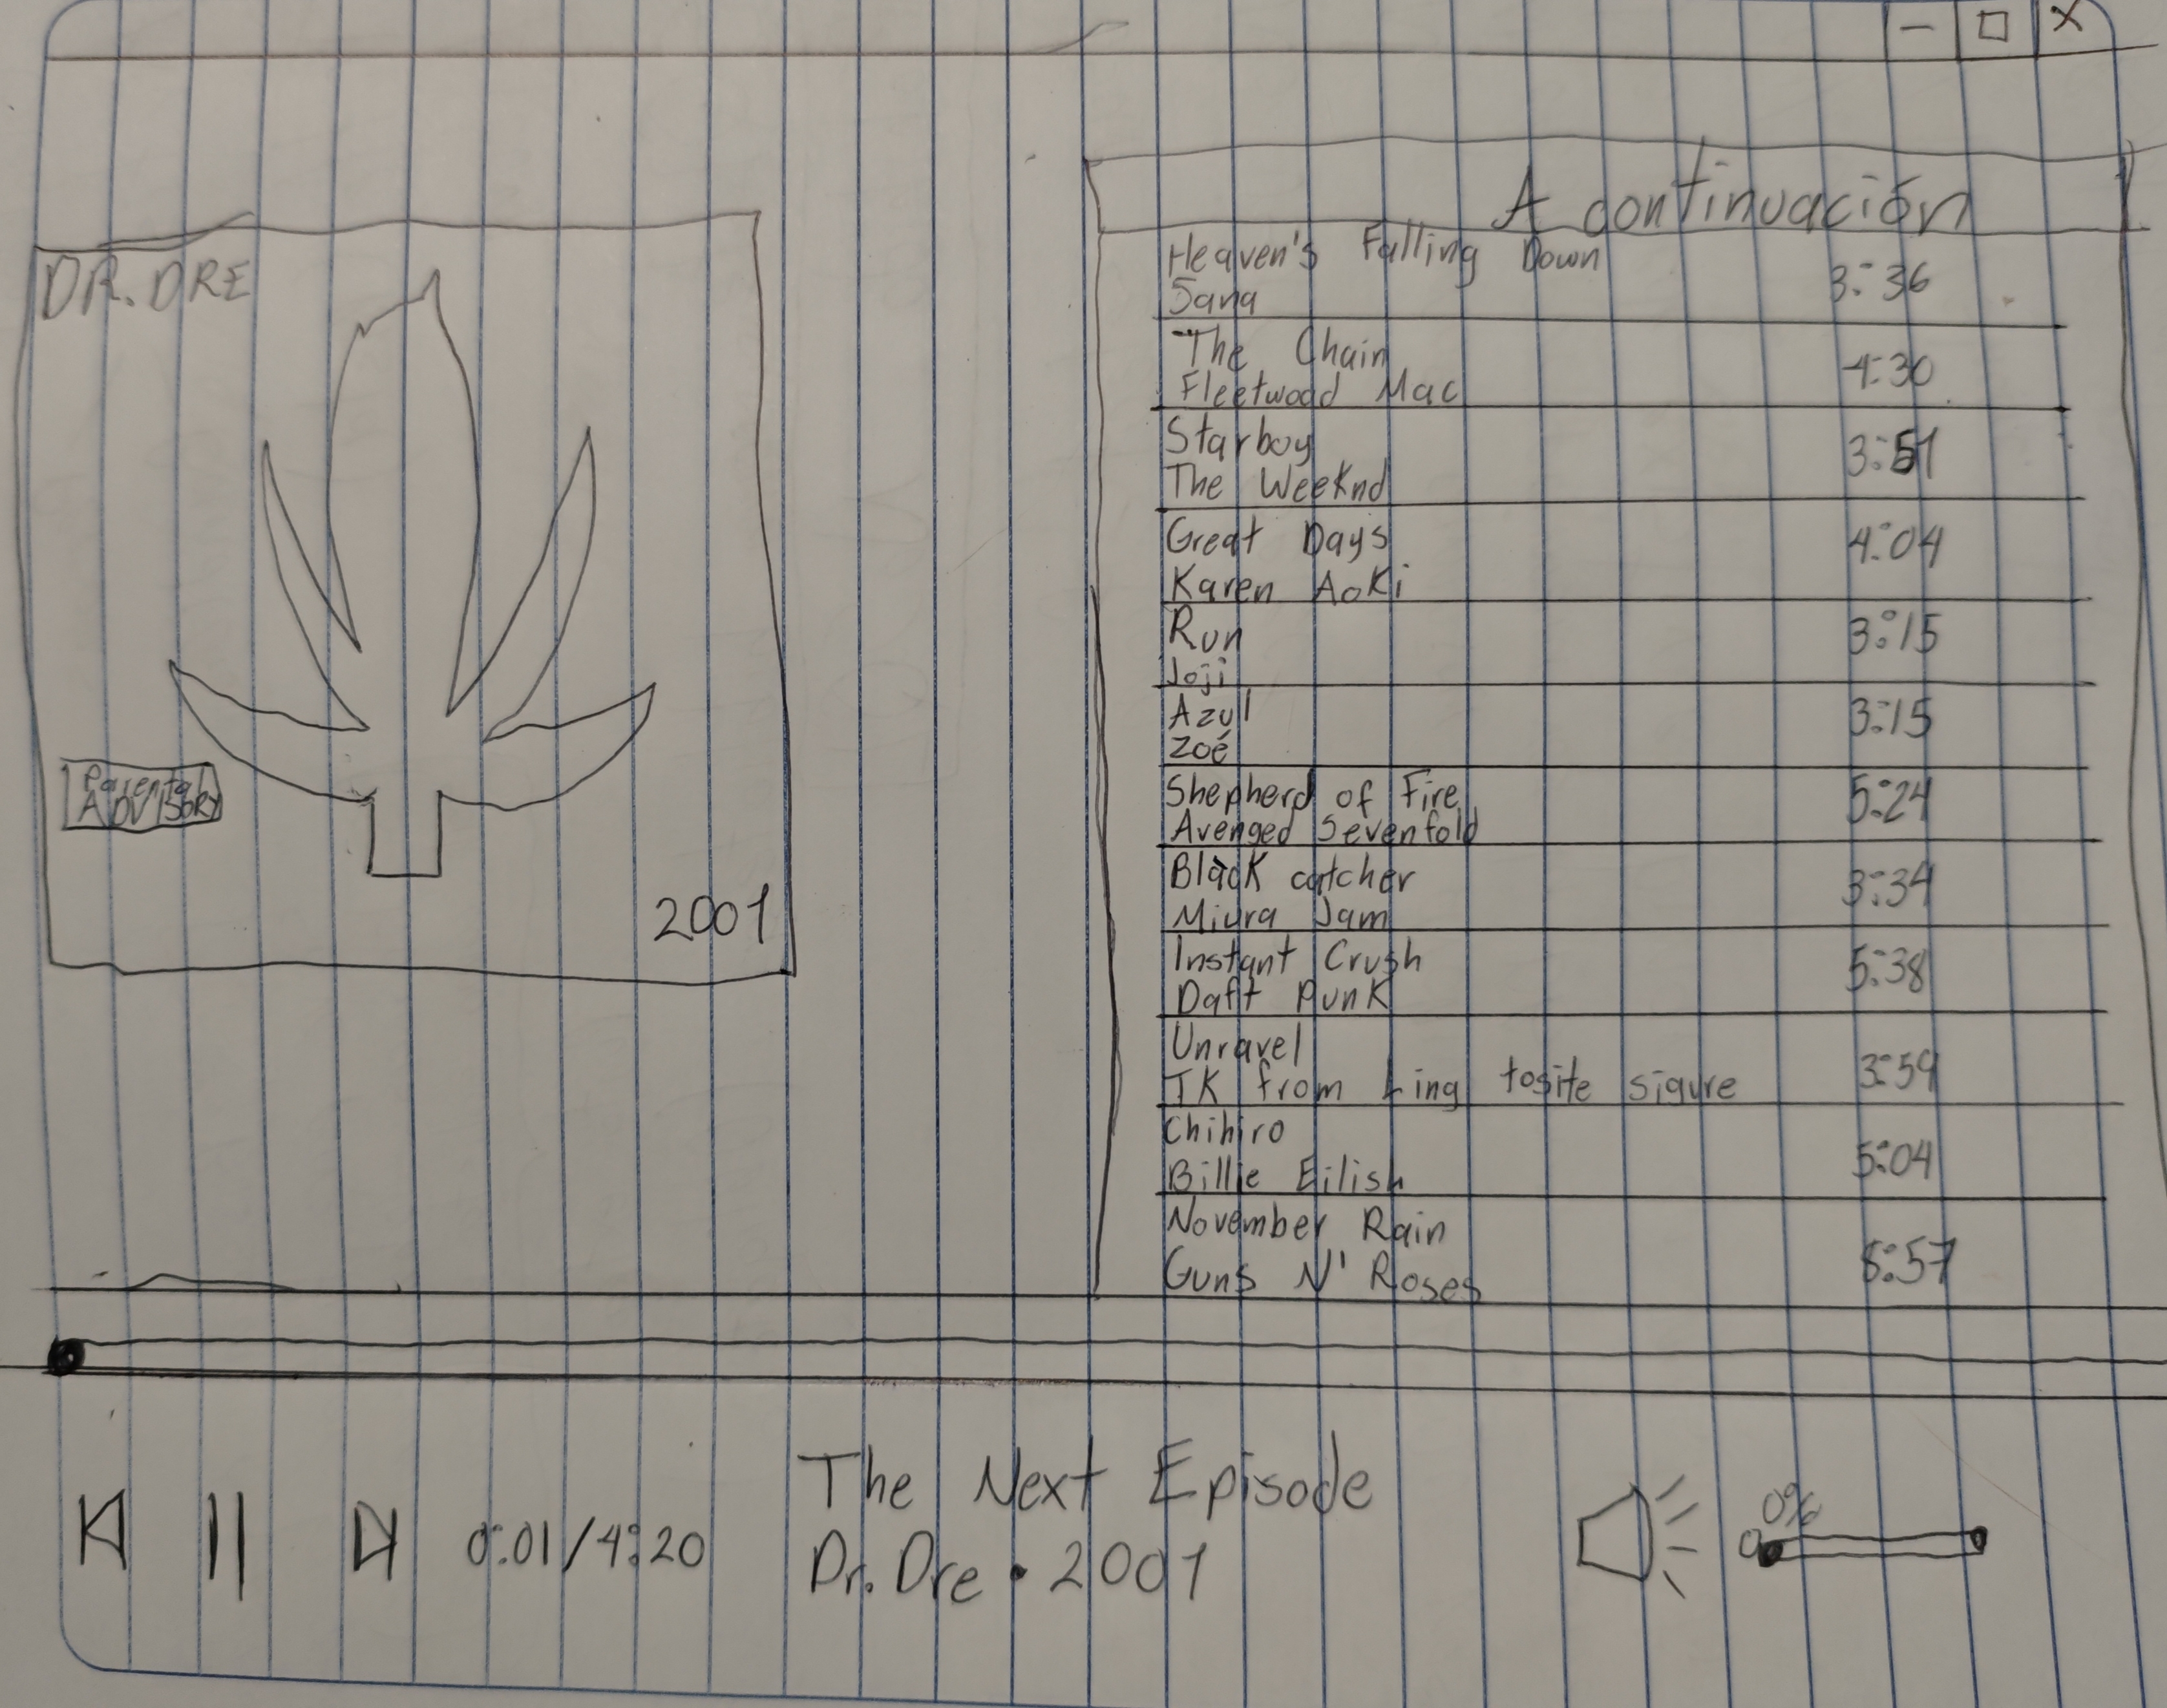
\includegraphics[width=0.38\textwidth]{interfazDibujo.jpg}
    \caption{Boceto inicial de la distribución de la ventana principal.}
\end{figure}

\subsection{Modelo de datos y reglas de importación}
La base de datos conserva las entidades definidas en \texttt{rolas.sql}. La tabla \texttt{types} establece las clasificaciones Persona, Grupo y Desconocido. La tabla \texttt{performers} representa al intérprete asociado a una canción; \texttt{persons} y \texttt{groups} guardan los datos particulares de cada tipo, mientras que \texttt{in\_group} relaciona personas con grupos. La tabla \texttt{albums} conserva el nombre, el año y la ruta del directorio del álbum, y \texttt{rolas} almacena los datos de las pistas y la ruta hacia cada archivo MP3.

El minero acepta una ruta a un archivo MP3 o a un directorio. Cuando recibe un directorio, lo recorre de forma recursiva para localizar archivos MP3. Para cada archivo se leen los metadatos y se comprueba si su ruta ya está registrada. Si la canción ya existe, se omite para no sobrescribir los cambios que el usuario haya realizado desde la interfaz. Los archivos que no cumplen con el formato ID3v2.4.0 requerido se descartan.

La asociación de álbumes se realiza utilizando el nombre del álbum presente en los metadatos y los nombres de los directorios superiores. Si se encuentra un directorio cuyo nombre coincide con el álbum, se registra su ruta; si no hay coincidencia, la canción se conserva sin álbum asociado. Esta regla se incorporó como una condición adicional para relacionar las pistas con las carpetas que las contienen. La duración se obtiene durante la lectura, pero no se almacena en SQLite.

\subsection{Arquitectura general del sistema}
El sistema tiene dos puntos de entrada. En la aplicación gráfica, el usuario interactúa con \texttt{VentanaPrincipal}, que reúne la barra de herramientas, el buscador, la vista de lista o galería, el panel de portada y los controles de reproducción. Los controladores conectan las acciones de la interfaz con los servicios y los objetos de acceso a datos. El botón de importación permite seleccionar un directorio e iniciar el servicio compartido de importación.

El segundo punto de entrada es el minero independiente. Este recibe desde la terminal la ruta de un archivo MP3 o de un directorio y delega el trabajo a la misma lógica de importación utilizada por la interfaz. El procesamiento utiliza la exploración de directorios y la lectura de metadatos con TagLib; después, la información se registra mediante los repositorios que acceden a SQLite.

La consulta de información sigue el camino inverso: los controladores solicitan datos a los DAO y estos consultan la base de datos. Los resultados se entregan al modelo de canciones y se muestran en la interfaz. La reproducción constituye un flujo separado de la importación: \texttt{Controlador\allowbreak{}RepUI} coordina los controles visuales y \texttt{Controlador\allowbreak{}Reproduccion} encapsula el uso de \texttt{QMediaPlayer} y \texttt{QAudioOutput}.

\begin{figure}[H]
    \centering
    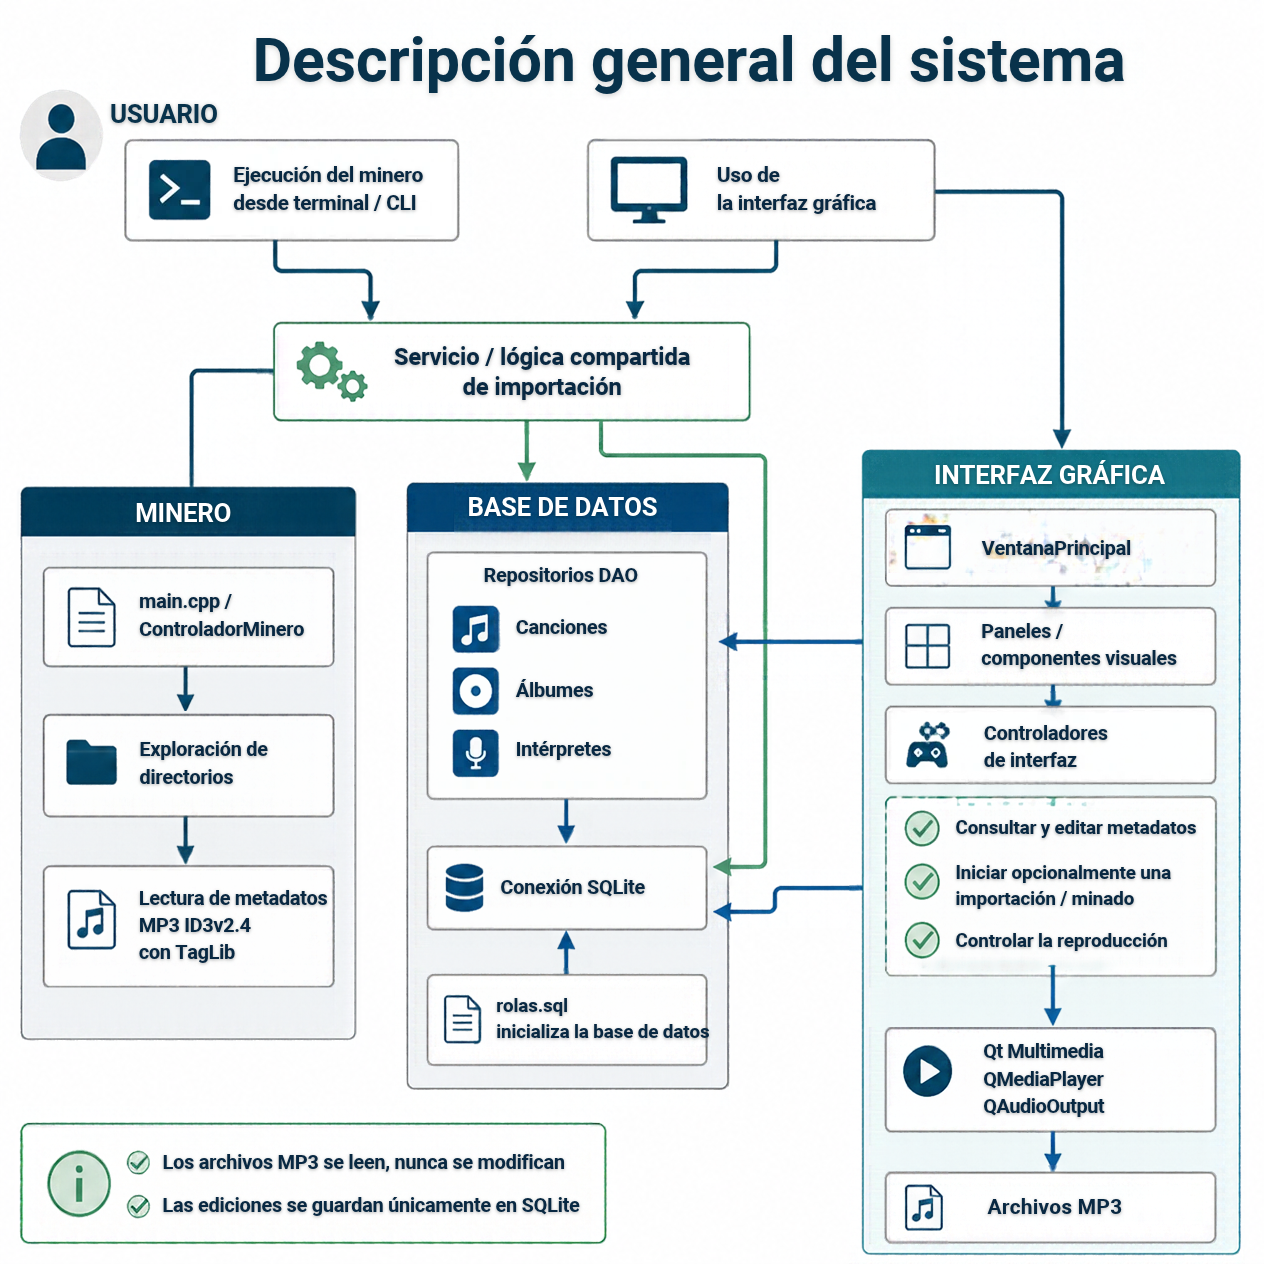
\includegraphics[width=0.64\textwidth]{diagramaGeneral.png}
        \caption{Arquitectura general del sistema.}
\end{figure}

\subsection{Operaciones principales}
Las operaciones más representativas y la parte del sistema que las atiende se resumen en el siguiente cuadro.

\begin{table}[H]
    \centering
    \begin{tabular}{|p{3.6cm}|p{10.4cm}|}
        \hline
        Importar música & La interfaz o el minero de terminal inician el mismo proceso de exploración, lectura y registro. \\ \hline
        Buscar canciones & La interfaz filtra la biblioteca por título, artista, álbum y año. \\ \hline
        Reproducir & Permite iniciar, pausar, cambiar de pista, ajustar el volumen y mover la posición de reproducción. \\ \hline
        Editar canciones & Modifica los datos de una pista y guarda los cambios en SQLite. \\ \hline
        Administrar álbumes & Permite modificar el nombre, el año y la ruta registrada del álbum. \\ \hline
        Administrar intérpretes & Permite registrar y editar personas, grupos e integrantes, incluso cuando no hay canciones asociadas. \\ \hline
        Cambiar de vista & Muestra la biblioteca como lista o galería de portadas. \\ \hline
    \end{tabular}
\end{table}

\subsection{Patrones y criterios de diseño}

\textbf{Data Access Object (DAO).} El patrón más importante utilizado en el proyecto es Data Access Object. Su propósito es separar las consultas y modificaciones de SQLite de las ventanas y controladores que necesitan esos datos. En lugar de construir sentencias SQL dentro de cada componente visual, la interfaz delega las operaciones a clases especializadas. Esto permite que los formularios trabajen con operaciones del dominio musical sin conocer los detalles de preparación de sentencias o asociación de parámetros.

Los principales objetos de esta capa son \texttt{Rolas}, que consulta las canciones; \texttt{EdicionCanciones}, que modifica los datos de las pistas; \texttt{EdicionAlbumes}, que consulta y actualiza álbumes; \texttt{EdicionInterpretes}, que administra personas, grupos e integrantes; y \texttt{CrearInterpretes}, que registra nuevos intérpretes. \texttt{RepositorioMusical} coordina operaciones relacionadas con la importación, como comprobar rutas existentes y resolver intérpretes y álbumes. Estos objetos utilizan \texttt{ConexionSQLite} para acceder a la base de datos.

\textbf{Separación inspirada en MVC.} La interfaz sigue una organización inspirada en Modelo-Vista-Controlador. Las ventanas y paneles representan la vista; \texttt{Canciones}, derivado de \texttt{QAbstractTableModel}, proporciona los datos que consumen las vistas; y los controladores conectan las acciones del usuario con los servicios y los DAO. Esta separación evita que la ventana principal concentre la importación, la edición, las consultas y el control del audio.

\textbf{RAII y administración de recursos.} La conexión SQLite y las sentencias preparadas se administran mediante punteros inteligentes y liberadores personalizados. \texttt{ConexionSQLite} mantiene el manejador de la base de datos en un \texttt{std::unique\_ptr} cuyo liberador cierra la conexión; las sentencias preparadas se liberan mediante \texttt{sqlite3\_finalize}. Así, los recursos se liberan al salir del alcance correspondiente, incluso si una operación termina por error.

\textbf{Sentencias preparadas y transacciones.} Las consultas que reciben datos variables utilizan sentencias preparadas y parámetros enlazados en lugar de concatenar directamente valores en la sentencia SQL. Las operaciones que modifican varias filas o entidades relacionadas utilizan transacciones: se inicia con \texttt{BEGIN IMMEDIATE}, se confirman los cambios con \texttt{COMMIT} si todo termina correctamente y se utiliza \texttt{ROLLBACK} cuando ocurre un error. Esto evita conservar modificaciones parciales durante la importación o la edición de álbumes e intérpretes.

\textbf{Señales, slots y ejecución asíncrona.} Qt utiliza señales y slots para comunicar cambios entre componentes, por ejemplo, para reaccionar a los clics, actualizar la posición de reproducción y reflejar el estado de \texttt{QMediaPlayer} en los controles visuales. Este mecanismo tiene una relación conceptual con Observer, pues permite notificar eventos a otros componentes. La importación iniciada desde la interfaz utiliza \texttt{QtConcurrent::run} y se supervisa con \texttt{QFutureWatcher}, evitando bloquear el hilo principal mientras se procesan los archivos.

\subsection{Diagramas de clases y secuencia}
El diagrama de clases agrupa las clases principales según los directorios del proyecto. En \texttt{interfazGrafica} se encuentran las ventanas, paneles, modelos y controladores que coordinan la interacción con el usuario; en \texttt{minero} se concentran los componentes encargados de explorar directorios y leer los metadatos; y en \texttt{baseDatos} se encuentran los repositorios DAO y la conexión con SQLite. Las relaciones muestran cómo colaboran estos componentes para importar, consultar y modificar la información de la biblioteca.

El diagrama de secuencia representa la importación iniciada desde la interfaz: selección del directorio, ejecución asíncrona, exploración, lectura de metadatos y registro en SQLite. También muestra las condiciones para omitir rutas ya registradas y archivos que no cumplen con ID3v2.4.0.
\begin{figure}[H]
    \centering
    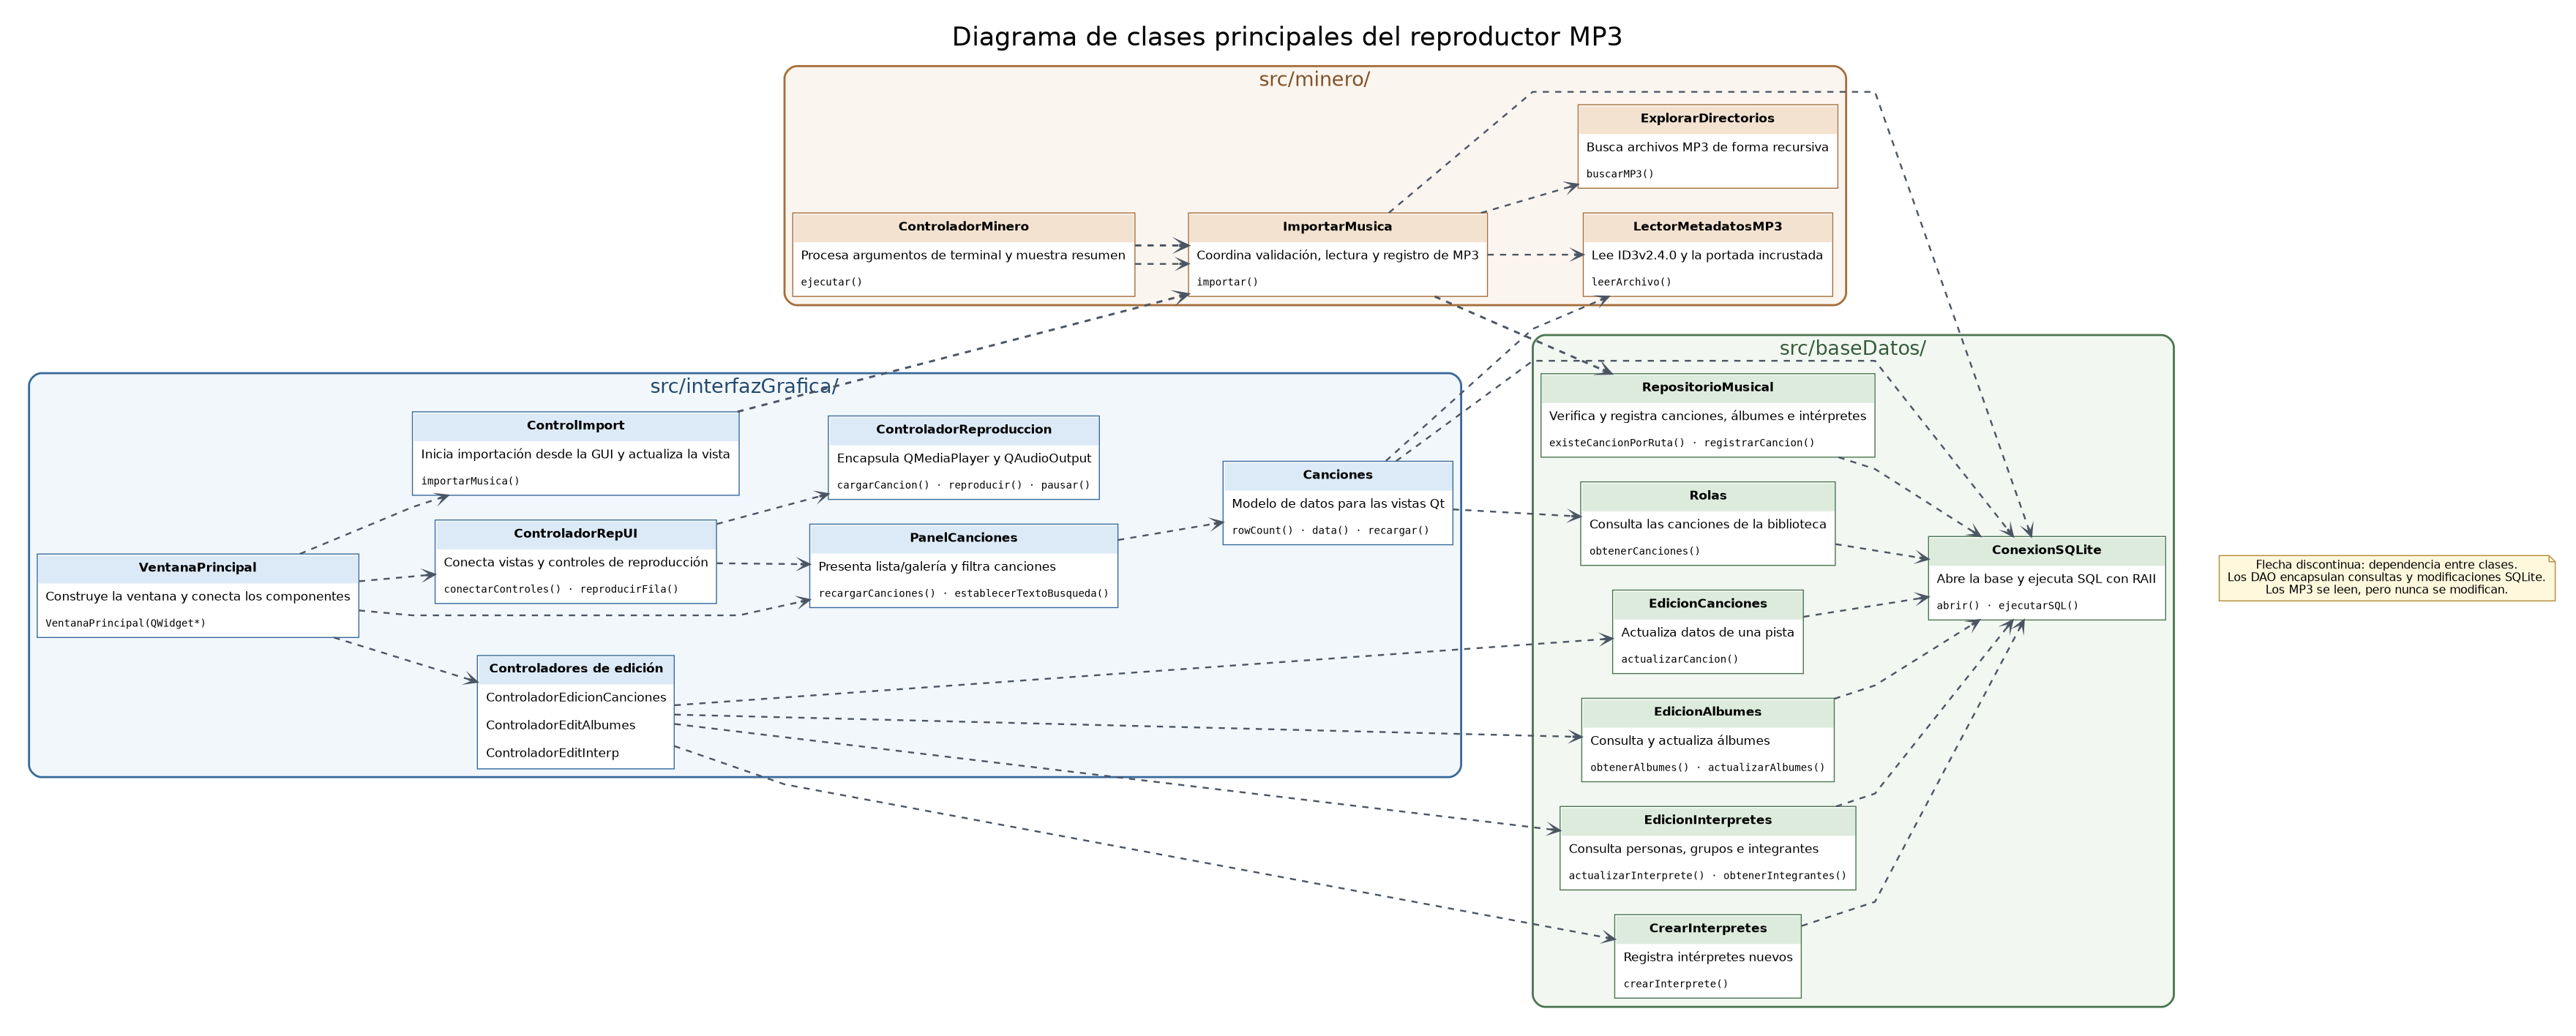
\includegraphics[width=\textwidth,
    height=0.43\textheight]{diagrama_clases.png}
    \caption{Diagrama de clases principales y sus dependencias.}
\end{figure}

\begin{figure}[H]
    \centering
    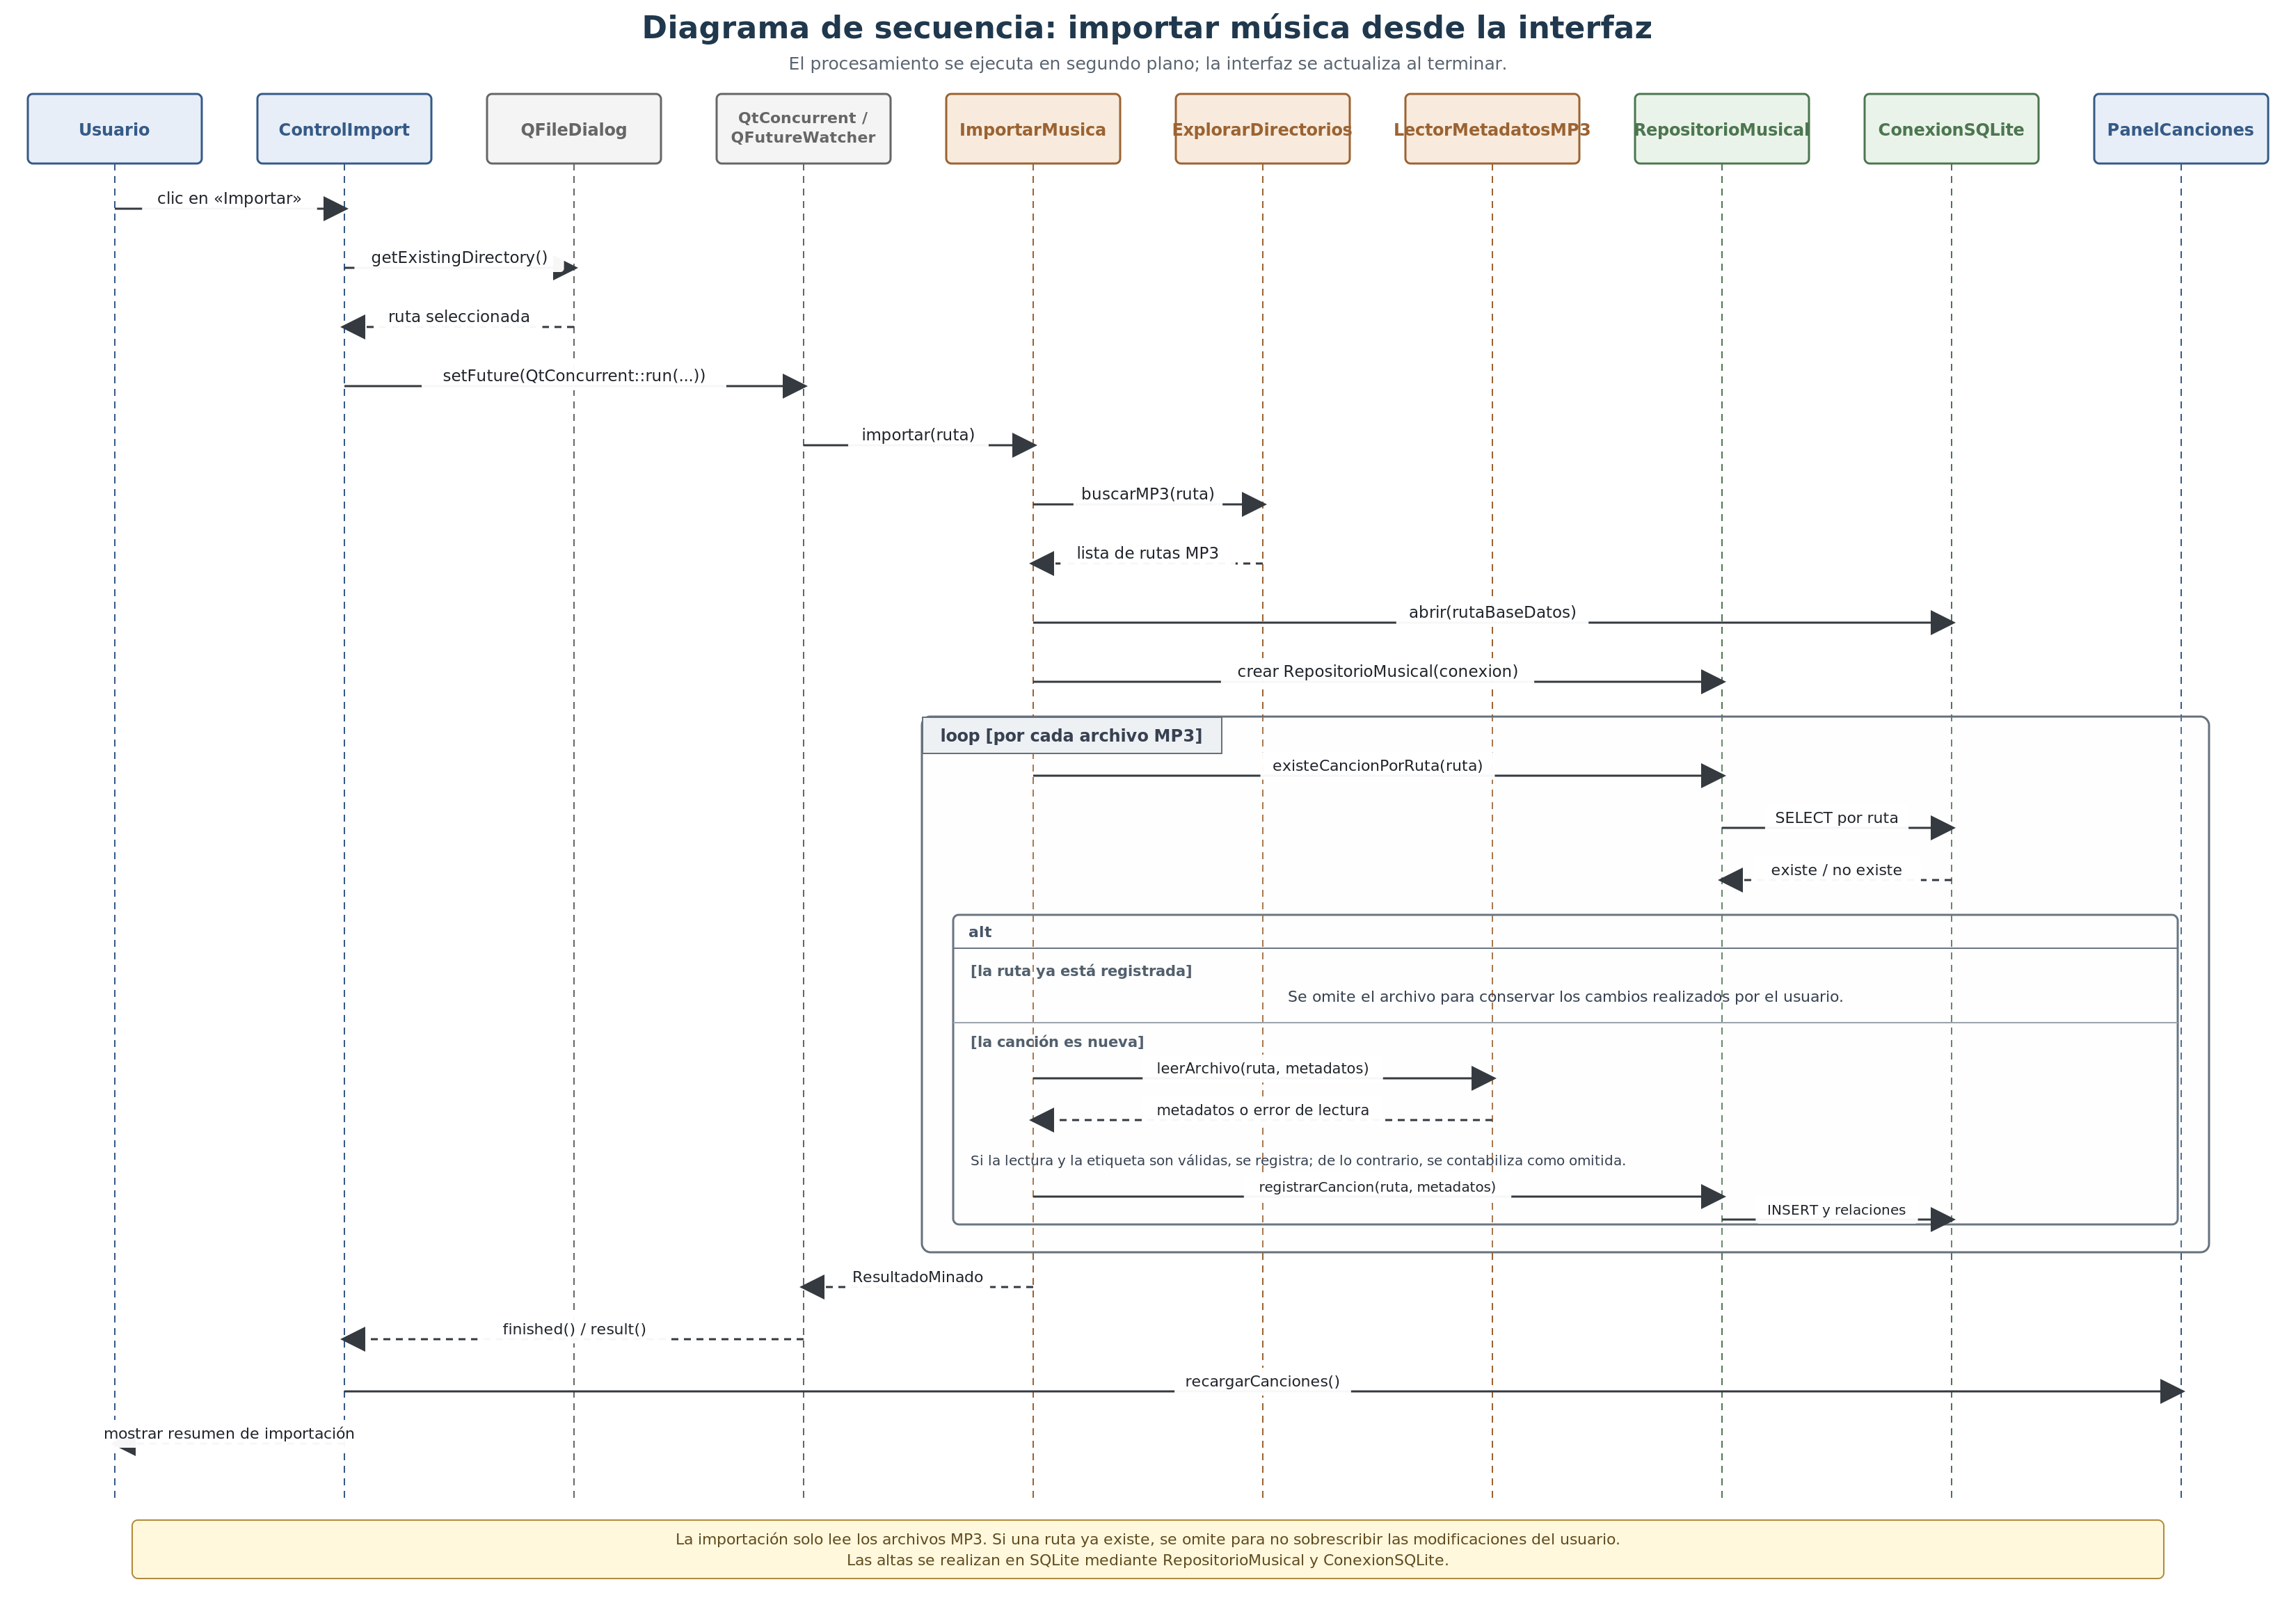
\includegraphics[width=\textwidth,
    height=0.42\textheight]{secuencia_importacion.png}
    \caption{Diagrama de secuencia de la importación de música desde la interfaz gráfica.}
\end{figure}

\section{Implementación}
\subsection{Tecnologías utilizadas}
Las principales tecnologías utilizadas se resumen en el siguiente cuadro.

\begin{table}[H]
    \centering
    \begin{tabular}{|p{3.2cm}|p{10.8cm}|}
        \hline
        C++17 & Lenguaje utilizado para desarrollar el minero, la persistencia y la interfaz. \\ \hline
        Qt 6 & Widgets para la interfaz, Multimedia para reproducir audio y Concurrent para ejecutar la importación en segundo plano. \\ \hline
        TagLib & Lectura de etiquetas ID3v2.4.0 y de información de los archivos MP3. \\ \hline
        SQLite3 & Almacenamiento de canciones, álbumes, intérpretes y relaciones entre personas y grupos. \\ \hline
        FFmpeg & Backend multimedia utilizado mediante la instalación de Qt Multimedia seleccionada para las pruebas. \\ \hline
        Meson y Ninja & Configuración y compilación del proyecto. \\ \hline
    \end{tabular}
\end{table}

\subsection{Minero e importación}
El minero utiliza un explorador de directorios para localizar archivos MP3 y TagLib para leer sus etiquetas. Entre los datos obtenidos se encuentran el título, artista, álbum, año, número de pista, género y las imágenes incrustadas compatibles. Los archivos que no cumplen con el requisito ID3v2.4.0 se descartan. Si una ruta ya se encuentra registrada, se omite para conservar las modificaciones hechas desde la interfaz.

La aplicación gráfica permite iniciar la importación desde un selector de directorio. El proceso se ejecuta con \texttt{QtConcurrent::run} y un \texttt{QFutureWatcher} recibe el resultado para actualizar la biblioteca al finalizar. La misma lógica puede ejecutarse de forma independiente desde la terminal.

\subsection{Interfaz gráfica y reproducción}
La interfaz utiliza Qt Widgets y el modelo/vista de Qt. \texttt{VentanaPrincipal} organiza la barra superior, el panel de portada, la lista o galería y el panel inferior de reproducción. \texttt{Canciones}, derivado de \texttt{QAbstractTableModel}, proporciona los datos que muestran las vistas. La búsqueda filtra la biblioteca por título, artista, álbum y año.

Para reproducir una canción, \texttt{Controlador\allowbreak{}RepUI} obtiene su ruta y delega la carga a \texttt{Controlador\allowbreak{}Reproduccion}. Las señales del reproductor actualizan la barra de progreso y la información de la canción.

También se implementan las acciones anterior, siguiente, pausa, volumen, silencio y avance automático al terminar una pista.

La portada visible da prioridad a una imagen personalizada almacenada por la aplicación. Si no existe, se intenta leer la imagen frontal incrustada en el MP3. Las imágenes personalizadas se guardan fuera de los archivos musicales, en directorios separados para canciones e intérpretes.

\subsection{Edición de canciones, álbumes e intérpretes}
La edición de canciones actualiza el título, intérprete, álbum y año de la pista seleccionada. El año de la canción se almacena en \texttt{rolas.year}, mientras que el año general del álbum se conserva en \texttt{albums.year}; son datos distintos y pueden modificarse de manera independiente.

La administración de intérpretes permite clasificar un registro como persona, grupo o desconocido. También permite registrar una persona aunque no interprete ninguna canción y crear grupos sin integrantes iniciales. Los integrantes se administran mediante la relación \texttt{in\_group}; al agregarlos, se comprueba que correspondan a personas registradas. La administración de álbumes permite modificar su nombre, año y ruta asociada, sin mover ni renombrar físicamente los directorios.

\subsection{Requerimientos, compilación y ejecución}
El proyecto se desarrolló y probó en Linux Mint de arquitectura x86\_64. Se requiere un compilador compatible con C++17, Meson, Ninja, pkg-config, TagLib, SQLite3 y Qt 6 con los módulos Widgets, Multimedia y Concurrent. El entorno de referencia utilizó Qt 6.12.0 y el backend FFmpeg 9.0.1 disponible en Qt Multimedia. La fuente Press Start 2P utilizada en algunos encabezados es opcional; si no está instalada, la interfaz utiliza una fuente alternativa.

Desde el directorio raíz del proyecto, y en la misma terminal donde se configuró la instalación seleccionada de Qt, se compila mediante:
\begin{verbatim}
meson setup build-qt612
meson compile -C build-qt612
\end{verbatim}
Si el directorio de compilación ya existe y no se cambió la instalación de Qt, normalmente basta con ejecutar \texttt{meson compile -C build-qt612}. Los ejecutables generados son:
\begin{itemize}
    \item Interfaz gráfica: \texttt{build-qt612/src/interfazGrafica/reproductor}.
    \item Minero independiente: \texttt{build-qt612/src/minero/minero}.
\end{itemize}

La base de datos debe inicializarse una sola vez antes del primer uso. Esto no significa que sea necesario minar una carpeta antes de abrir la interfaz: la importación de música está disponible desde el propio reproductor. Para inicializarla se ejecuta:
\begin{verbatim}
./build-qt612/src/minero/minero --inicializar-bd
\end{verbatim}
Después se puede abrir la aplicación gráfica con:
\begin{verbatim}
./build-qt612/src/interfazGrafica/reproductor
\end{verbatim}
Para importar desde la terminal, el minero acepta la ruta de un directorio o de un único archivo MP3:
\begin{verbatim}
./build-qt612/src/minero/minero "$HOME/Música"
./build-qt612/src/minero/minero "/ruta/a/cancion.mp3"
\end{verbatim}

\subsection{Organización del proyecto}
El código fuente se divide en directorios según la responsabilidad de cada componente. La organización principal se resume a continuación.

\begin{table}[H]
    \centering
    \begin{tabular}{|p{5.1cm}|p{8.9cm}|}
        \hline
        \texttt{src/baseDatos/} & Conexión SQLite, inicialización, rutas y esquema de la base de datos. \\ \hline
        \texttt{src/baseDatos/repositorio/} & Consultas y modificaciones de canciones, álbumes e intérpretes mediante objetos DAO. \\ \hline
        \texttt{src/minero/} & Punto de entrada del minero, exploración de directorios, lectura de metadatos y servicio de importación. \\ \hline
        \texttt{src/interfazGrafica/} & Ventanas, paneles, modelos, controladores, servicios de imágenes y reproducción. \\ \hline
    \end{tabular}
\end{table}

\section{Problemas encontrados y soluciones}

\subsection{Problema 1}
El primer problema de este proyecto fue que no encontraba información sobre cómo realizar un minero, ni proyectos que ya hubieran hecho uno o una mínima ayuda en algún lugar sobre un minero de archivos MP3 con ID3v2.4.0.
\subsubsection{Solución}
La solución fue que, afortunadamente, terminé llegando a la documentación de TagLib para tratar de utilizarla. Menciono que terminé llegando porque la mayoría de las soluciones a mis problemas provinieron de Reddit, pero, para no citar Reddit, simplemente utilizaba las documentaciones a las que me redirigían por los comentarios.

\subsection{Problema 2}
El archivo SQL que mandó Canek. Tuve muchos problemas para entender cómo utilizar ese archivo de \texttt{rolas.sql}.
\subsubsection{Solución}
Me hubiera gustado que se explicara un poco más sobre el archivo, porque leer la documentación de SQL para entender a qué se refería cada cosa fue algo muy tedioso.

\subsection{Problema 3}
Archivos MP3. La escasez de archivos para probar el proyecto era algo que afectaba directamente al buscador, por ejemplo, o a la posibilidad de probar el registro de canciones en directorios con nombres determinados y comprobar que así aparecieran en la interfaz. No solo es que no tuviera apenas archivos para probar, sino que cada descargador en línea no incluía los metadatos o los archivos estaban etiquetados con ID3v2.3, lo que los hacía inútiles para las pruebas. Era frustrante no poder probar el proyecto adecuadamente por la falta de archivos.
\subsubsection{Solución}
En un día de locura absoluta, después de dos horas de buscar algo que me ayudara a resolver esto, logré encontrar una solución bastante buena. Me voy a extender detallando esto porque fue muy importante para el desarrollo del proyecto.

Pensé en utilizar un descargador genérico y simplemente modificar todos los campos vacíos a mano. Como todavía no contaba con la interfaz y solo tenía el minero, pensaba hacerlo directamente en los archivos. Gracias a Reddit terminé descargando \texttt{beets}, que era lo que me iba a ayudar a modificar un MP3 directamente; sin embargo, me di cuenta de que iba a desperdiciar demasiado tiempo en esto.

Terminé utilizando SpotyMate para descargar los MP3 con metadatos. El problema era que eran ID3v2.3 y, en un momento de iluminación, se me ocurrió transformarlos a ID3v2.4. Combinando \texttt{beets} con un script de Python, pude recorrer todo mi directorio de Música para identificar los archivos que eran ID3v2.3 y transformarlos a ID3v2.4.

Al final, gasté todo un día solo para esto, pero definitivamente valió la pena porque me permitió tener muchísima variedad de archivos de prueba funcionales para el proyecto.

\subsection{Problema 4}
Toda la interfaz. No hay un problema específico. Simplemente, cada vez que la compilaba algo salía mal, se me movían cosas, no funcionaba lo que programaba o de plano me tardaba mucho en lograr que compilara.
\subsubsection{Solución}
En un inicio seguí tutoriales de YouTube para los botones de reproducción, reproducir audio y mostrar las canciones. Prácticamente después de esto fue cuestión de volver a buscar en Reddit cosas que me fueran de ayuda con Qt, ya que la cantidad de cosas que se pueden utilizar es tan inmensa que buscar lo que necesitas era algo casi imposible de realizar en el poco tiempo que tenía.

La verdad, ni siquiera hay una solución exacta a este problema; todo fue cuestión de prueba y error XD.

\subsection{Problema 5}
El problema de compatibilidad. De nuevo, creo que voy a explicar esto de forma muy detallada.

Durante el desarrollo se utilizó inicialmente Qt 6.4.2, versión proporcionada por los repositorios de Linux Mint. Sin embargo, al probar la reproducción y el cambio de canciones comenzaron a aparecer advertencias relacionadas con Qt Multimedia y GLib. El error más frecuente era:
\begin{verbatim}
GLib-GObject-CRITICAL:
g_object_unref: assertion 'G_IS_OBJECT (object)' failed
\end{verbatim}

Al revisar la salida de Qt Multimedia se observó que el sistema tenía disponibles los backends FFmpeg y GStreamer, pero estaba cargando GStreamer. Las advertencias aparecían después de conectar la salida de audio y se repetían al cambiar de canción.

Para identificar el origen se probaron ambos backends por separado. GStreamer podía reproducir archivos directamente mediante \texttt{gst-launch}, sin presentar las mismas advertencias. Sin embargo, al utilizarlo desde Qt Multimedia aparecía nuevamente el error de GLib. Esto apuntaba a un problema en la interacción entre Qt Multimedia y el backend GStreamer, aunque no fue posible determinar una causa interna definitiva.

También se probó FFmpeg desde Qt Multimedia. Aunque el backend podía cargarse y permitía cambiar de pista, en las pruebas realizadas no conseguía reproducir el audio ni actualizar correctamente el progreso. En algunos intentos se obtuvo el error \texttt{ResourceError: Could not open file}. Por tanto, tampoco fue posible utilizarlo satisfactoriamente con la configuración inicial.

\subsubsection{Solución}
Ante esta situación se decidió instalar una versión independiente de Qt mediante Qt Online Installer. Se seleccionó Qt 6.12.0 y se utilizó el backend FFmpeg 9.0.1 como entorno de referencia para el proyecto. La instalación original de Qt 6.4.2 proporcionada por Linux Mint se mantuvo disponible, pero dejó de utilizarse para compilar y ejecutar el reproductor.

Para evitar que las herramientas mezclen componentes de ambas instalaciones, se configuraron las variables de entorno para utilizar Qt 6.12.0 de manera consistente:
\begin{verbatim}
export QT_ROOT="$HOME/Qt/6.12.0/gcc_64"
export PATH="$QT_ROOT/bin:$PATH"
export PKG_CONFIG_PATH="$QT_ROOT/lib/pkgconfig${PKG_CONFIG_PATH:+:$PKG_CONFIG_PATH}"
export LD_LIBRARY_PATH="$QT_ROOT/lib${LD_LIBRARY_PATH:+:$LD_LIBRARY_PATH}"
export QT_PLUGIN_PATH="$QT_ROOT/plugins"
\end{verbatim}

La versión de los módulos utilizados se puede comprobar mediante:
\begin{verbatim}
pkg-config --modversion Qt6Widgets Qt6Multimedia Qt6Concurrent
\end{verbatim}

Los tres módulos deben corresponder a la misma instalación. Si se cambia la versión de Qt después de configurar el proyecto, es necesario volver a generar el directorio de compilación de Meson para evitar que conserve las rutas de las dependencias anteriores:
\begin{verbatim}
rm -rf build-qt612
meson setup build-qt612
meson compile -C build-qt612
\end{verbatim}

De esta manera se estableció un entorno de desarrollo consistente, evitando mezclar bibliotecas, encabezados y complementos multimedia de distintas instalaciones de Qt.

\section{Conclusiones}
El comienzo del desarrollo fue complicado, pero afortunadamente pude completar la parte del minero y la base de datos sin muchas complicaciones, ya que gran parte de esto era cuestión de leer la documentación de lo que iba a utilizar.

Los consejos que daba Canek durante las clases fueron clave para cambiar el rumbo de mi proyecto para bien; muchas cosas se facilitaron gracias a su ayuda.

La peor parte, sin duda, fue todo lo relacionado con la interfaz gráfica. Había que leer demasiadas cosas y un mínimo cambio mal hecho podía ocasionar muchos problemas en ella. La mayoría de los problemas que tuve que enfrentar en este proyecto fueron por culpa de la interfaz gráfica y, de no ser por el paro, probablemente no hubiera terminado a tiempo.

\section{Referencias}

\footnotesize
\begin{itemize}
    \item ID3.org. \textit{ID3v2.4.0 Structure}.
    \url{https://id3.org/id3v2.4.0-structure}

    \item ID3.org. \textit{ID3v2.4.0 Frames}.
    \url{https://id3.org/id3v2.4.0-frames}

    \item TagLib. \textit{API Documentation}.
    \url{https://taglib.org/api/}

    \item SQLite. \textit{C/C++ Interface}.
    \url{https://www.sqlite.org/cintro.html}

    \item SQLite. \textit{Opening a Database Connection}.
    \url{https://www.sqlite.org/c3ref/open.html}

    \item SQLite. \textit{Binding Values to Prepared Statements}.
    \url{https://www.sqlite.org/c3ref/bind_blob.html}

    \item SQLite. \textit{Result Values From a Query}.
    \url{https://www.sqlite.org/c3ref/column_blob.html}

    \item SQLite. \textit{Prepared Statement Object}.
    \url{https://www.sqlite.org/c3ref/stmt.html}

    \item SQLite. \textit{Compiling an SQL Statement}.
    \url{https://www.sqlite.org/c3ref/prepare.html}

    \item SQLite. \textit{Evaluating an SQL Statement}.
    \url{https://www.sqlite.org/c3ref/step.html}

    \item SQLite. \textit{Resetting a Prepared Statement}.
    \url{https://www.sqlite.org/c3ref/reset.html}

    \item SQLite. \textit{Finalizing a Prepared Statement}.
    \url{https://www.sqlite.org/c3ref/finalize.html}

    \item SQLite. \textit{Closing a Database Connection}.
    \url{https://www.sqlite.org/c3ref/close.html}

    \item SQLite. \textit{Executing SQL Statements}.
    \url{https://www.sqlite.org/c3ref/exec.html}

    \item SQLite. \textit{Last Insert Row ID}.
    \url{https://www.sqlite.org/c3ref/last_insert_rowid.html}

    \item SQLite. \textit{Counting Modified Rows}.
    \url{https://www.sqlite.org/c3ref/changes.html}

    \item SQLite. \textit{Error Codes and Messages}.
    \url{https://www.sqlite.org/c3ref/errcode.html}

    \item SQLite. \textit{Memory Allocation}.
    \url{https://www.sqlite.org/c3ref/free.html}

    \item SQLite. \textit{Foreign Key Support}.
    \url{https://www.sqlite.org/foreignkeys.html}

    \item SQLite. \textit{Transactions}.
    \url{https://www.sqlite.org/lang_transaction.html}

    \item SQLite. \textit{PRAGMA Statements}.
    \url{https://www.sqlite.org/pragma.html}

    \item Qt. \textit{Qt Core}.
    \url{https://doc.qt.io/qt-6/qtcore-index.html}

    \item Qt. \textit{Qt GUI}.
    \url{https://doc.qt.io/qt-6/qtgui-index.html}

    \item Qt. \textit{Qt Widgets}.
    \url{https://doc.qt.io/qt-6/qtwidgets-index.html}

    \item Qt. \textit{QAbstractTableModel}.
    \url{https://doc.qt.io/qt-6/qabstracttablemodel.html}

    \item Qt. \textit{QAbstractItemView}.
    \url{https://doc.qt.io/qt-6/qabstractitemview.html}

    \item Qt. \textit{Model/View Programming}.
    \url{https://doc.qt.io/qt-6/model-view-programming.html}

    \item Qt. \textit{QMainWindow}.
    \url{https://doc.qt.io/qt-6/qmainwindow.html}

    \item Qt. \textit{QWidget}.
    \url{https://doc.qt.io/qt-6/qwidget.html}

    \item Qt. \textit{QDialog}.
    \url{https://doc.qt.io/qt-6/qdialog.html}

    \item Qt. \textit{QPushButton}.
    \url{https://doc.qt.io/qt-6/qpushbutton.html}

    \item Qt. \textit{QLineEdit}.
    \url{https://doc.qt.io/qt-6/qlineedit.html}

    \item Qt. \textit{QTableView}.
    \url{https://doc.qt.io/qt-6/qtableview.html}

    \item Qt. \textit{Layouts y QFormLayout}.
    \url{https://doc.qt.io/qt-6/layout.html}
    \url{https://doc.qt.io/qt-6/qformlayout.html}

    \item Qt. \textit{QSortFilterProxyModel}.
    \url{https://doc.qt.io/qt-6/qsortfilterproxymodel.html}

    \item Qt. \textit{QDate y QDateEdit}.
    \url{https://doc.qt.io/qt-6/qdate.html}
    \url{https://doc.qt.io/qt-6/qdateedit.html}

    \item Qt. \textit{QFileDialog}.
    \url{https://doc.qt.io/qt-6/qfiledialog.html}

    \item Qt. \textit{QPixmap y QImage}.
    \url{https://doc.qt.io/qt-6/qpixmap.html}
    \url{https://doc.qt.io/qt-6/qimage.html}

    \item Qt. \textit{Signals and Slots}.
    \url{https://doc.qt.io/qt-6/signalsandslots.html}

    \item Qt. \textit{Qt Concurrent}.
    \url{https://doc.qt.io/qt-6/qtconcurrent-index.html}

    \item Qt. \textit{QFutureWatcher}.
    \url{https://doc.qt.io/qt-6/qfuturewatcher.html}

    \item Qt. \textit{Qt Multimedia}.
    \url{https://doc.qt.io/qt-6/qtmultimedia-index.html}

    \item Qt. \textit{QMediaPlayer}.
    \url{https://doc.qt.io/qt-6/qmediaplayer.html}

    \item Qt. \textit{QAudioOutput}.
    \url{https://doc.qt.io/qt-6/qaudiooutput.html}

    \item Qt. \textit{QSlider}.
    \url{https://doc.qt.io/qt-6/qslider.html}

    \item cppreference. \textit{C++ Standard Library}.
    \url{https://en.cppreference.com/w/cpp/standard_library.html}

    \item cppreference. \textit{std::filesystem}.
    \url{https://en.cppreference.com/w/cpp/filesystem}
    \item cppreference. \textit{std::unique\_ptr}.
    \url{https://en.cppreference.com/w/cpp/memory/unique_ptr}

\end{itemize}

\end{document}